\documentclass[]{article}
\usepackage{lmodern}
\usepackage{natbib}
\usepackage[figuresright]{rotating}
\usepackage{amsmath,amssymb}
\usepackage{bbm}
%\usepackage{subfigure}
\usepackage{graphicx}
\usepackage{subcaption}
\captionsetup{compatibility=false}
\font\myfont=cmr12 at 15pt
\renewcommand{\baselinestretch}{1.0}
\setlength{\baselineskip}{20pt}
\usepackage{amssymb,amsmath}
\usepackage{ifxetex,ifluatex}
\usepackage{}
\linespread{1.6} 
\usepackage{fixltx2e} % provides \textsubscript
\ifnum 0\ifxetex 1\fi\ifluatex 1\fi=0 % if pdftex
  \usepackage[T1]{fontenc}
  \usepackage[utf8]{inputenc}
\else % if luatex or xelatex
  \ifxetex
    \usepackage{mathspec}
  \else
    \usepackage{fontspec}
  \fi
  \defaultfontfeatures{Ligatures=TeX,Scale=MatchLowercase}
\fi
% use upquote if available, for straight quotes in verbatim environments
\IfFileExists{upquote.sty}{\usepackage{upquote}}{}
% use microtype if available
\IfFileExists{microtype.sty}{%
\usepackage{microtype}
\UseMicrotypeSet[protrusion]{basicmath} % disable protrusion for tt fonts
}{}
\usepackage[margin=1in]{geometry}
\usepackage{hyperref}
\urlstyle{same}  % don't use monospace font for urls
\usepackage{graphicx,grffile}
\makeatletter
\def\maxwidth{\ifdim\Gin@nat@width>\linewidth\linewidth\else\Gin@nat@width\fi}
\def\maxheight{\ifdim\Gin@nat@height>\textheight\textheight\else\Gin@nat@height\fi}
\makeatother
% Scale images if necessary, so that they will not overflow the page
% margins by default, and it is still possible to overwrite the defaults
% using explicit options in \includegraphics[width, height, ...]{}
\setkeys{Gin}{width=\maxwidth,height=\maxheight,keepaspectratio}
\IfFileExists{parskip.sty}{%
\usepackage{parskip}
}{% else
\setlength{\parindent}{0pt}
\setlength{\parskip}{6pt plus 2pt minus 1pt}
}
\setlength{\emergencystretch}{3em}  % prevent overfull lines
\providecommand{\tightlist}{%
  \setlength{\itemsep}{0pt}\setlength{\parskip}{0pt}}
\setcounter{secnumdepth}{5}
% Redefines (sub)paragraphs to behave more like sections
\ifx\paragraph\undefined\else
\let\oldparagraph\paragraph
\renewcommand{\paragraph}[1]{\oldparagraph{#1}\mbox{}}
\fi
\ifx\subparagraph\undefined\else
\let\oldsubparagraph\subparagraph
\renewcommand{\subparagraph}[1]{\oldsubparagraph{#1}\mbox{}}
\fi

%%% Use protect on footnotes to avoid problems with footnotes in titles
\let\rmarkdownfootnote\footnote%
\def\footnote{\protect\rmarkdownfootnote}

%%% Change title format to be more compact
\usepackage{titling}
\usepackage{inputenc}
\usepackage[english]{babel}

\setlength{\parindent}{2em}
\setlength{\parskip}{1em}

% Create subtitle command for use in maketitle
\providecommand{\subtitle}[1]{
  \posttitle{
    \begin{center}\large#1\end{center}
    }
}

\usepackage{xcolor}
\newcommand{\highlight}[1]{\textcolor{red}{#1}}
\newcommand{\alex}[1]{\textcolor{blue}{#1}}



\setlength{\droptitle}{-2em}
 \title{{\myfont Bayesian Inference for Cox Proportional Hazard Models with Partial Likelihoods, Semi-Parametric Covariate Effects and Correlated Observations}}
    \pretitle{\vspace{\droptitle}\centering\huge}
  \posttitle{\par}
    \preauthor{\centering\large\emph}
  \postauthor{\par}
      \predate{\centering\large\emph}
  \postdate{\par}
    \date{07/02/2020}
    \author{Ziang Zhang, Alex Stringer, Patrick Brown, Jamie Stafford}


\begin{document}
	
\maketitle

\begin{abstract}
We develop an approximate Bayesian inference methodology for the Cox Proportional Hazards model for survival data with partial likelihood, semi-parametric covariate effects and correlated survival times. The use of Bayesian inference yields model-based uncertainty quantification of the smoothness parameters and between-group standard deviations. The use of partial likelihood avoids smoothness assumptions on the baseline hazard, leading to improved inferences over current methods for approximate Bayesian inference for this model (INLA). A simulation study demonstrates the superior accuracy of our approximations over existing methods when the baseline hazard is not smooth. Analysis of two benchmark datasets demonstrates the use of our method to yield full posterior uncertainty for the smoothness of the semi-parametric effect and the between-subject standard deviation without making assumptions about the baseline hazard. An R package implementing our method will be released publicly.
\end{abstract}


\section{Introduction}
Survival data consists of times to an event of interest such as mortality or morbidity.  When analysing survival data, the Cox proportional hazards (Cox PH) model is a common choice. The Cox PH model assumes that any two subjects' event hazards are proportional as a function of time, with the ratio depending on covariate effects which are modelled as unknown linear or smooth functions and inferred from the observed data. Event times may be correlated within the sample, for example when the response is time to kidney failure for the left and right kidneys from the same subject. Inference is often conducted using a partial likelihood which does not depend on the baseline hazard, avoiding the need to make assumptions about its form. Further, the use of Bayesian inference with the Cox PH model is desirable as this yields model-based estimation and uncertainty quantification for the smoothness of the covariate effects, and in the case of correlated survival times, the between-group standard deviations. However, existing methods for approximate Bayesian inference based on Integrated Nested Laplace Approximations (INLA) \citet{inla} cannot be applied to the Cox PH model with partial likelihood. Application of the INLA methodology to the Cox PH model requires restrictive smoothness assumptions to be made about the smoothness of the baseline hazard \citep{inlacoxph}.

Recently, \citet{casecross} developed an approximate Bayesian inference methodology for a model involving a partial likelihood. Their methodology includes smooth covariate effects and yields full posterior uncertainty for the smoothness parameters, an improvement over existing frequentist methods based on Generalized Additive Models (GAMs). By applying a strategy similar to INLA they demonstrate up to an order of magnitude improvement in computation time when compared to sampling-based approaches to Bayesian inference. However, the partial likelihood they consider is simpler than that of the Cox PH model.

In this paper we extend the approximate Bayesian inference methodology of \citet{casecross} to the Cox proportional hazard models with partial likelihood. Our methodology accommodates semi-parametric smoothing effects and correlation between observed survival times. We demonstrate improved accuracy over INLA in simulations where the assumption of a smooth baseline hazard is violated. Through two data analysis examples we demonstrate the use of our method for model-based estimation and uncertainty quantification for the smoothness of effects and between-subject standard deviations, without making assumptions about the baseline hazard.

The remainder of this paper is organized as follows. In \S\ref{sec:prelim}, we describe the Cox proportional hazard model and the partial likelihood function, and review the approximate Bayesian inference methodology of \citet{casecross}. In \S\ref{sec:method}, we describe our proposed methodology. In \S\ref{sec:example} we illustrate our methodology in a simulation study and through the analysis of two benchmark datasets. We conclude in \S\ref{sec:discussion} with a discussion.



\section{Preliminaries}\label{sec:prelim}
\subsection{Cox Proportional Hazard Model}
Let T denote a random variable representing the time to some event, supported on the interval $[0,\infty)$. For $t\in[0,\infty)$ the \textit{hazard function} $h(t)$ of $T$ is defined as:
\begin{equation}\begin{aligned}\label{eqn:hazard}
h(t) = \lim_{s\to 0} \frac{P(t\le T \le t+s |T\ge t)}{s}
\end{aligned}\end{equation}
\alex{Add to this section: notation for the observations that accomodates censoring. Redefine an ``observation'' to be the pair $(Y_{ij},d_{ij})$. Add a note that ``ties are handled according to the method of Breslow (cite)''. Also, I think we should denote the total number of datapoints as $N = \sum_{i=1}^{n}n_{i}$, and define this here.} Suppose we observe $i = 1,\ldots,n$ groups each with $j = 1,\ldots,n_{i}$ survival times. For example, we may observe $n$ subjects with $n_{i}$ measurements per subject. Denote the random variable representing the $j^{th}$ survival time in the $i^{th}$ group by $Y_{ij}$, and denote the survival times by $y = \left\{y_{ij}: i = 1,\ldots,n; j = 1,\ldots,n_{i} \right\}$. When there are some survival data in a data-set that are not observed exactly, we call these observations $censored$. Right-censoring is a common case of censoring when some survival times are only known to be longer than some specific times. For example, if the observation $y_{ij}$ is right-censored, then the only information available for $Y_{ij}$ is that $Y_{ij} > y_{ij}$. We will focus on this type of censoring in this paper.
Define $h_{ij}(t)$ to be the hazard function for random variable $Y_{ij}$. The Cox PH model assumes \citep{coxph}
\begin{equation}\begin{aligned}\label{eqn:CoxHazardModel}
h_{ij}(t) = h_0(t)\text{exp}(\eta_{ij})
\end{aligned}\end{equation}
where $h_0(t)$ is an unknown baseline hazard function that does not depend on the covariates. The additive predictor $\eta = \left\{ \eta_{ij}: i = 1,\ldots,n; j = 1,\ldots,n_{i}\right\}$ links the covariates for observation $y_{ij}$ to the observed survival time:
\begin{equation}\begin{aligned}\label{eqn:eta}
\eta_{ij} =x_{ij}^{T}\beta+\sum_{q=1}^{r} \gamma_q(u_{q_{ij}}) +\xi_{i}
\end{aligned}\end{equation}
Here $x_{ij}$ is a $p$-dimensional vector of covariates that are modelled as having linear associations with the log-hazard, and $\beta = (\beta_{1},\ldots,\beta_{p})$ are regression coefficients. The $u_{q} = \left\{u_{qij}: i = 1,\ldots,n; j = 1,\ldots,n_{i} \right\}, q = 1,\ldots,r$ are covariate vectors whose association with the log-hazard is modelled non-parametrically through unknown smooth functions $\gamma_1,\ldots,\gamma_r$. The vector of group intercepts $\xi = \left\{ \xi_{i}: i=1,\ldots,n\right\}$, referred to as ``frailty'' coefficients in the context of survival analysis \citep{frailty}, are included to model correlation between survival times coming from the same group $i$.

Inference is carried out via a partial likelihood function. Define the \textit{risk set} $R_{ij} = \left\{k,l : y_{kl} \geq y_{ij}\right\}$. The partial likelihood can be written as follows: \alex{I removed all extra text from this paragraph. The censoring notation should already be defined. Make sure to modify the partial likelihood function appropriately, as discussed.}
\begin{equation}\begin{aligned}\label{eqn:partial}
\pi(y|\eta) &= \prod_{i=1}^{n}\prod_{j=1}^{r_{i}} \bigg\{\frac{\exp[\eta_{ij}]}{{\sum_{l,k\in R_{ij}}^{}\exp[\eta_{lk}]}}\bigg \} \\
&= \prod_{i=1}^{n}\prod_{j=1}^{r_{i}} \bigg\{\frac{1}{{1 + \sum_{l,k\in R_{ij} , (l,k) \neq (i,j)}\exp[\Delta_{lk,ij}]}}\bigg \} \\
\end{aligned}\end{equation}
where $\Delta_{lk,ij} = \eta_{lk} - \eta_{ij}$. Note that $h_{0}(t)$ does not appear in the partial likelihood, and hence inference may be carried out in the absence of assumptions about $h_{0}(t)$. Also note that this partial likelihood can be written in the following form:
\begin{equation}\begin{aligned}\label{eqn:whyINLAfail1}
\pi(y|\eta) &= \prod_{i=1}^{n}\prod_{j=1}^{r_{i}} \pi(y_{ij}|\eta)
\end{aligned}\end{equation}
while in order for a model to be compatible with INLA, its likelihood must have the form:
\begin{equation}\begin{aligned}\label{eqn:whyINLAfail2}
\pi(y|\eta) &= \prod_{i=1}^{n}\prod_{j=1}^{n_{i}} \pi(y_{ji}|\eta_{ij})
\end{aligned}\end{equation}
\citet{inlacoxph} use a data-augmentation trick to write their likelihood in the form (\ref{eqn:whyINLAfail2}), but do not use the partial likelihood. Their method requires assumptions about the smoothness of the baseline hazard.

\subsection{Approximate Bayesian Inference}

To perform Bayesian inference for this model, we specify prior distributions for all unknowns. A joint Gaussian prior distribution with fixed covariance matrix is used for $\beta \sim  \text{N}(0,\Sigma_\beta)$. We follow \citet{casecross} and use $\Sigma_{\beta} = \sigma^{2}_{\beta}I_{p}$, with $\sigma^{2}_{\beta} = 1000$. The group intercepts $\xi = \left\{ \xi_{i}, i = 1\ldots n\right\}$ are given independent Gaussian priors $\xi_{i} | \theta \stackrel{iid}{\sim} \text{N}(0,\sigma_{\xi}),i = 1,\ldots,n$ where $\sigma_{\xi}$ is the between-group standard deviation. Let $U_{q} = \{U_{ql};l = 1, ...., m_q\}$ be the ordered vector of \textit{unique} values of covariate $u_q,q = 1,\ldots,r$; often these values are set by the user by discretizing the covariate $u_q$ into $m_q$ pre-specifed bins. To infer the infinite-dimensional parameters $\gamma_{q},q = 1,\ldots,r$, we approximate each by a piecewise constant function with jumps at the $U_{ql}$, which we denote as $\gamma(U_{ql}) = \Gamma_{ql}$. We define the vectors of function values $\Gamma_{q} = \left\{ \Gamma_{q1},\ldots,\Gamma_{qm_{q}}\right\}$ and these are given a joint Gaussian distribution $\Gamma_{q}|\theta\sim\text{N}\left[ 0,\Sigma_{q}(\sigma_{q})\right]$ which is parametrized through its precision matrix $\Sigma_{q}(\sigma_{q})$ depending on a variance parameter $\sigma_{q}$. A popular choice which we adopt in our analysis is the second-order random walk model \citep{rw2}. Let $\Gamma = (\Gamma_{1},\ldots,\Gamma_{r})$; we have that $\Gamma|\sigma_{1},\ldots,\sigma_{q}\sim\text{N}\left( 0,\Sigma^{-1}_{\Gamma}\right)$ with $\Sigma^{-1}_{\Gamma} = \text{diag}\left[ \Sigma_{1}^{-1}(\sigma_{1}),\ldots,\Sigma_{r}^{-1}(\sigma_{r})\right]$. Finally, define the variance parameter vector $\theta = (\theta_{0},\ldots,\theta_{r})$ where $\theta_{q} = -2\log\sigma_{q},q = 1,\ldots,r$, and $\theta_{0} = -2\log\sigma_{\xi}$. The variance parameters are given prior distribution $\theta \sim \pi(\theta)$. 

For computational purposes, we follow \citet{inla} and \citet{casecross} to add a small random noise on the linear predictor, redefining: 
\begin{equation}\begin{aligned}\label{eqn:etaredefine}
\eta_{ij} =x_{ij}^{T}\beta+\sum_{q=1}^{r} \gamma_q(u_{q_{ij}}) +\xi_{i} + \epsilon_{ij}
\end{aligned}\end{equation}
where $\epsilon_{ij} \stackrel{iid}{\sim} \text{N}(0,\tau^{-1})$ for some large, fixed $\tau$. We follow the established default used by \citet{inla} and \citet{casecross} and set $\tau = \exp(12)$ so the addition of the $\epsilon$ noise does not significantly change the inferential result. In particular, \citet{casecross} demonstrate in their Web Appendix E that choices of $\tau$ in the broad range of $\exp(2),\ldots,\exp(14)$ yield virtually identical inferences and similar running times. Further redefine $\Delta_{lk,ij} = \eta_{lk} - \eta_{ij}$ in terms of the augmented additive predictors (\ref{eqn:etaredefine}), and note that since $\Delta_{lk,ij} = \Delta_{11,ij} - \Delta_{11,lk}$ for every $(i,j,l,k)$, the entire partial likelihood (\ref{eqn:partial}) depends on $\eta$ only through the vector $\Delta = \left\{\Delta_{11,ij}: i = 1,\ldots,n; j = 1,\ldots,n_{i} \right\}$. For the remainder of the paper we reflect this in our notation, writing $\pi(y|\Delta) \equiv \pi(y|\eta)$ and defining the log-likelihood $\ell(\Delta; y) = \log\pi(y|\Delta)$.

Define $W = \left(\Delta, \Gamma,\beta, \xi \right)$ which we refer to as the \textit{mean parameters} and let $\text{dim}(W) = m$. Our model specifies $W|\theta\sim\text{N}\left[ 0,Q^{-1}_{\theta}\right]$. An expression for $Q_{\theta}$ is given in \S\ref{sec:method} and a derivation is given in Web Appendix A. Our main inferential interest is to obtain the marginal posterior distributions of the mean parameters:
\begin{equation}\begin{aligned}\label{eqn:interestedQuat3}
\pi(W_{k}|y) = \int \pi(W_i|y,\theta) \pi(\theta|y) d\theta, k = 1,\ldots,m  \\
\end{aligned}\end{equation}
These are used for point estimates and uncertainty quantification of the mean parameters, which often include the effects of primary interest. We are also interested in the joint posterior distributions of the variance parameters:
\begin{equation}\begin{aligned}\label{eqn:interestedQuat1}
\pi(\theta|y) = \frac{\int \pi(W,y,\theta) dW}{\int_{} \int_{} \pi(W,y,\theta) dW d\theta } \\
\end{aligned}\end{equation}
These are used for point estimates and uncertainty quantification of the variance parameters, and appear as integration weights in (\ref{eqn:interestedQuat3}). Of secondary inference is the joint posterior distribution of the mean parameters:
\begin{equation}\begin{aligned}\label{eqn:interestedQuat2}
\pi(W|y) = \int \pi(W|y,\theta) \pi(\theta|y) d\theta  \\
\end{aligned}\end{equation}
This appears primarily as an intermediate step in the calculation of the marginal posteriors (\ref{eqn:interestedQuat3}).

All of the quantities of interest (\ref{eqn:interestedQuat3}) -- (\ref{eqn:interestedQuat2}) depend on intractable high-dimensional integrals. \citet{casecross} utilize Gaussian and Laplace approximations combined with numerical quadrature to approximate each of these integrals accurately and efficiently. Their approximations take the form
\begin{equation}\begin{aligned}\label{eqn:integration}
\tilde{\pi}(W_{j}|y) &= \sum_{k=1}^{K}
\tilde{\pi}_{G}(W_{j}|y,\theta^{k})
\tilde{\pi}_{LA}(\theta^{k}|y)\delta_{k} \\
\tilde{\pi}(W|y) &= \sum_{k=1}^{K}
\tilde{\pi}_{G}(W|y,\theta^{k})
\tilde{\pi}_{LA}(\theta^{k}|y)\delta_{k} \\
\end{aligned}\end{equation}
For any fixed $\theta$, define
\begin{equation}\begin{aligned}\label{eqn:modeandhessian}
\widehat{W}_{\theta} = \left( \widehat{\Delta}_{\theta},\widehat{\Gamma}_{\theta},\widehat{\beta},\widehat{\xi}_{\theta}\right) &= \text{argmax}_{W}\log\pi(W|\theta,Y) \\ 
H_{\theta}(W) &= -\frac{\partial^{2}}{\partial W \partial W^{T}}\log\pi(W|\theta,Y) \\
v(\theta)_j^2 &= \left[H_\theta \left(\widehat{W}_{\theta}\right) ^ {-1} \right]_{jj}
\end{aligned}\end{equation}
To approximate the density,
\begin{equation}\begin{aligned}\label{eqn:condpost}
\pi(W|\theta,Y) \propto \exp\left\lbrace -\frac{1}{2}W^{T}Q_{\theta}W + \ell\left(\Delta;Y\right)\right\rbrace
\end{aligned}\end{equation}
a second-order Taylor expansion of $\log(W|\theta,Y)$ about $W = \widehat{W}_{\theta}$ gives a Gaussian approximation:
\begin{equation}\label{eqn:gaussianapprox}
\pi(W|\theta,Y) \approx \tilde{\pi}_{G}(W|y,\theta) \propto \text{exp}\left\{-\frac{1}{2} \left(W-\widehat{W}_{\theta} \right)^T H_\theta\left(\widehat{W}_{\theta}\right) \left(W-\widehat{W}_{\theta} \right) \right\} \\
\end{equation}
Direct integration of this Gaussian approximation yields a Gaussian approximation for the correnspoding marginal density:
\begin{equation}\label{eqb:marginalgaussianapprox}
\pi(W_{k}|\theta,Y) = \int\pi(W|\theta,Y)dW_{-k} \approx \tilde{\pi}_{G}(W_{k}|y,\theta) \propto\text{exp}\left\{-\frac{1}{2v(\theta)_j^2} \left(W_j-\widehat{W}_{\theta j} \right)^2 \right\}, k = 1,\ldots,m
\end{equation}
For the joint posterior of the variance parameters, the method of \citet{tierney} yields a Laplace approximation:
\begin{equation}\begin{aligned}\label{eqn:laplace}
\pi(\theta|Y) \approx \tilde{\pi}_{LA}(\theta|y) \propto \pi(\theta)\left\{\frac{\left|Q_{\theta}\right|}{\left|H_{\theta}\left(\widehat{W}_{\theta}\right)\right|}\right\}^{1/2}\exp\left\{ -\frac{1}{2}\widehat{W}_{\theta}^{T}Q_{\theta}\widehat{W}_{\theta} + \ell\left(\widehat{\Delta}_{\theta};y \right)\right\}
\end{aligned}\end{equation}
The Hessian matrix $H_{\theta}(W)$ has the form $H_{\theta}(W) = Q_{\theta} + C(W)$ where
\begin{equation*}
C(W) = -\frac{\partial^{2}}{\partial W\partial W^{T}}\ell(\Delta) = -\begin{pmatrix}
\frac{\partial^{2}\ell(\Delta;y)}{\partial\Delta\partial\Delta^{T}} & 0 & 0 \\
0 & 0 & 0 \\
0 & 0 & 0 \\
\end{pmatrix}
\end{equation*}
Because the partial likelihood takes the form (\ref{eqn:whyINLAfail1}), $C(W)$ has a dense structure. In contrast, \citet{inla} assume that the likelihood takes the form (\ref{eqn:whyINLAfail2}) which has $C(W) \equiv \text{diag}(c)$, and hence cannot fit the Cox PH model with partial likelihood. \citet{casecross} relax this assumption to allow $C(W)$ to have a block-diagonal structure; our work extends this to permit a fully dense $C(W)$. 

\section{Methodology}\label{sec:method}

In this section we construct the quantities necessary to implement the approximations (\ref{eqn:integration}), with a focus on computational considerations. We describe the novel approach taken to the optimization required to compute $\widehat{W}_{\theta}$, describing how we address the challenge of a dense $C(W)$.

\subsection{Precision Matrix}\label{subsec:Q} 

For fixed design matrices $A$, $B$ and $X$, we may write the additive predictor (\ref{eqn:etaredefine}) as:
\begin{equation}
\eta = A\Gamma + B\xi + X\beta + \epsilon
\end{equation}
where $\epsilon \sim \text{N}\left( 0,\tau^{-1}I_{N}\right)$.
\alex{Now, I think you were right to split $A$ and $B$. It makes our procedure look more novel. Do you have the corresponding formula for the $Q_{\theta}$ matrix? I have only done this for the no-eps methodology, in which it is trivial to add new terms. If you don't have it, I think the easiest way to derive it would be to take my old formula for $Q_{\theta}$ from the case crossover paper, replace $A$ with $(A:B)$ and $\Gamma$ with $(\Gamma,\xi)$, and expand it out. }
In \S\ref{sec:prelim}, it is shown that the partial likelihood function only depends on $\eta$ through $\Delta$ \alex{note: this is true for the vectors, but not true for the scalars as you put}. Hence the partial likelihood depends on $\Delta = D\eta$ where $D$ is an $(N -1) \times N $-dimensional matrix of rank $N -1$ \alex{see my note in section 2 about defining $N$. In general, whenever you find yourself writing a messy quantity more than once, consider defining a term for it.} The precision matrix is given by
\begin{equation}\label{eqn:precmat}
Q_{\theta} = \tau\begin{pmatrix}
\Lambda^{-1} & -\Lambda^{-1}DA & - \Lambda^{-1}DX \\
- A^{T}D^{T}\Lambda^{-1} & \frac{1}{\tau}\Sigma_{\Gamma}^{-1} +  A^{T}D^{T}\Lambda^{-1}DA &  A^{T}D^{T}\Lambda^{-1}DX \\
- X^{T}D^{T}\Lambda^{-1} &  X^{T}D^{T}\Lambda^{-1}DA & \frac{1}{\tau}\Sigma_{\beta}^{-1} +  X^{T}D^{T}\Lambda^{-1}DX \\
\end{pmatrix}
\end{equation}
\alex{we need to agree on whether or not to include $B$ and then modify this formula} where $\Lambda = DD^{T}$. Expressions for $D$ and $\Lambda^{-1}$ are given in Appendix A. The specific form of the partial likelihood and this differencing matrix allow estimation of the frailty coefficients $\xi_{i},i = 1,\ldots,n$. In contrast, these are not estimable in the model considered by \citet{casecross}.

\subsection{Optimization}\label{subsec:opt}

To compute the conditional mode $\hat{W}(\theta)$, we use trust region optimization \citep{trustoptim}. The objective function (\ref{eqn:modeandhessian}) is convex and high-dimensional, and hence trust region methods are well-suited to this problem. The Hessian of the objective function is $H_{\theta}(W) = Q_{\theta} + C(W)$. The non-zero block of $C(W)$ is fully dense in the Cox PH model with partial likelihood. The prior precision matrix $Q_{\theta}$ is also dense since $\Lambda^{-1}$ is. Since this density comes from $\Lambda^{-1}$, the Hessian $H_{\theta}(W)$ inherits the same sparsity pattern as $Q_{\theta}$.

To apply such methods when the Hessian of the objective function is dense, we utilize quasi-Newton updates inside the trust region procedure. Such updates use a low-rank approximation to $H_{\theta}(W)$ at each iteration and hence do not require evaluation of this matrix during optimization. While this can lead to more iterations than the method used by \citet{casecross}, we are able to optimize our objective function efficiently in the presence of a dense $H_{\theta}(W)$. 


\alex{note: I removed the paragraph on ties-- see our previous conversation. I think this can be reduced to a simple mention in the preliminaries.}

\subsection{Models for latent variables}

We use a second-order random walk (RW2) model for each $\Gamma_{q},q = 1\ldots r$ \citep{rw2}. These models usually contain an intercept $\beta_{0}$ and a \emph{sum-to-zero} constraint $\sum_{q=1}^{r}\Gamma_{q} = 0$, for identifiability of parameters. However, as in \citet{casecross}, an intercept itself is not identifiable when using the partial likelihood for inference, and the sum-to-zero constraint may not be applied. We instead fit the following modified RW2 model for each $q = 1,\ldots,r$:
\begin{equation}\begin{aligned}\label{eqn:rw2}
\Gamma_{q,l+1} - 2\Gamma_{q,l} + \Gamma_{q,l-1} &\overset{iid}{\sim}\text{N}\left( 0,\sigma^{2}_{q}\right), \\
\Gamma_{q,a} = 0,
\end{aligned}\end{equation}
where $a\in\mathbb{R}$ is some chosen reference value. This parametrization is identifiable under the partial likelihood and gives a clear interpretation of $\Gamma_{q,l}$ as the change in log-risk for an individual with covariate $u_{q,l}$ compared to an individual with covariate $u_{q,a}$. \alex{what is the second constraint you use? Two are needed for identifiability in RW2. Is this the part that you fix by adding the $vv^{T}$ onto the diagonal of the precision matrix?}


\section{Examples}\label{sec:example}

We will illustrate the accuracy of our method over INLA, and the ability of our method to yield full posterior uncertainty for the smoothness of the semi-parametric effect and between subject standard deviation, through a simulation study and two real data analysis examples.

\subsection{Simulation study}

To illustrate the accuracy of our method over INLA when the smoothness assumption for baseline hazard function is violated, we performed a simulation study. We generated $N = n = 400$ uncorrelated data points from a distribution with hazard function (\ref{eqn:hazard}). The baseline hazard $h_{0}(t)$ shown in Figure \ref{fig:simulation} and the additive predictor is $\eta_{i} = \gamma\left(u_{i}\right)$ with $\gamma(u) = 1.5 [ \text{sin}(0.8u) + 1 ]$. To generate the covariate $u$ we first generate $u_{1},\ldots,u_{n}\overset{iid}{\sim}\text{Unif}(0,1)$ \alex{confirm: what did you actually do here?}, and then discretized these values into 50 disjoint, evenly-spaced intervals. Further, we randomly censored $80$ observations. 

We fit a RW2 model using our procedure and the INLA software \citep{inla}. For INLA, we used their default first-order random walk model for the baseline hazard, run under its default settings. This implicitly assumes that $h_{0}(t)$ is smooth. In contrast, our procedure does not infer $h_{0}(t)$, and does not make assumptions about its smoothness. For the single variance parameter $\sigma$ we use an Exponential($\lambda$) prior with $\lambda$ chosen such that $\mathbb{P}\left( \sigma > 2.5\right) = 0.5$, corresponding to a penalized complexity prior \citep{pcprior}.

\begin{figure}[ht]
\centering
\subcaptionbox{baseline hazard function}{
	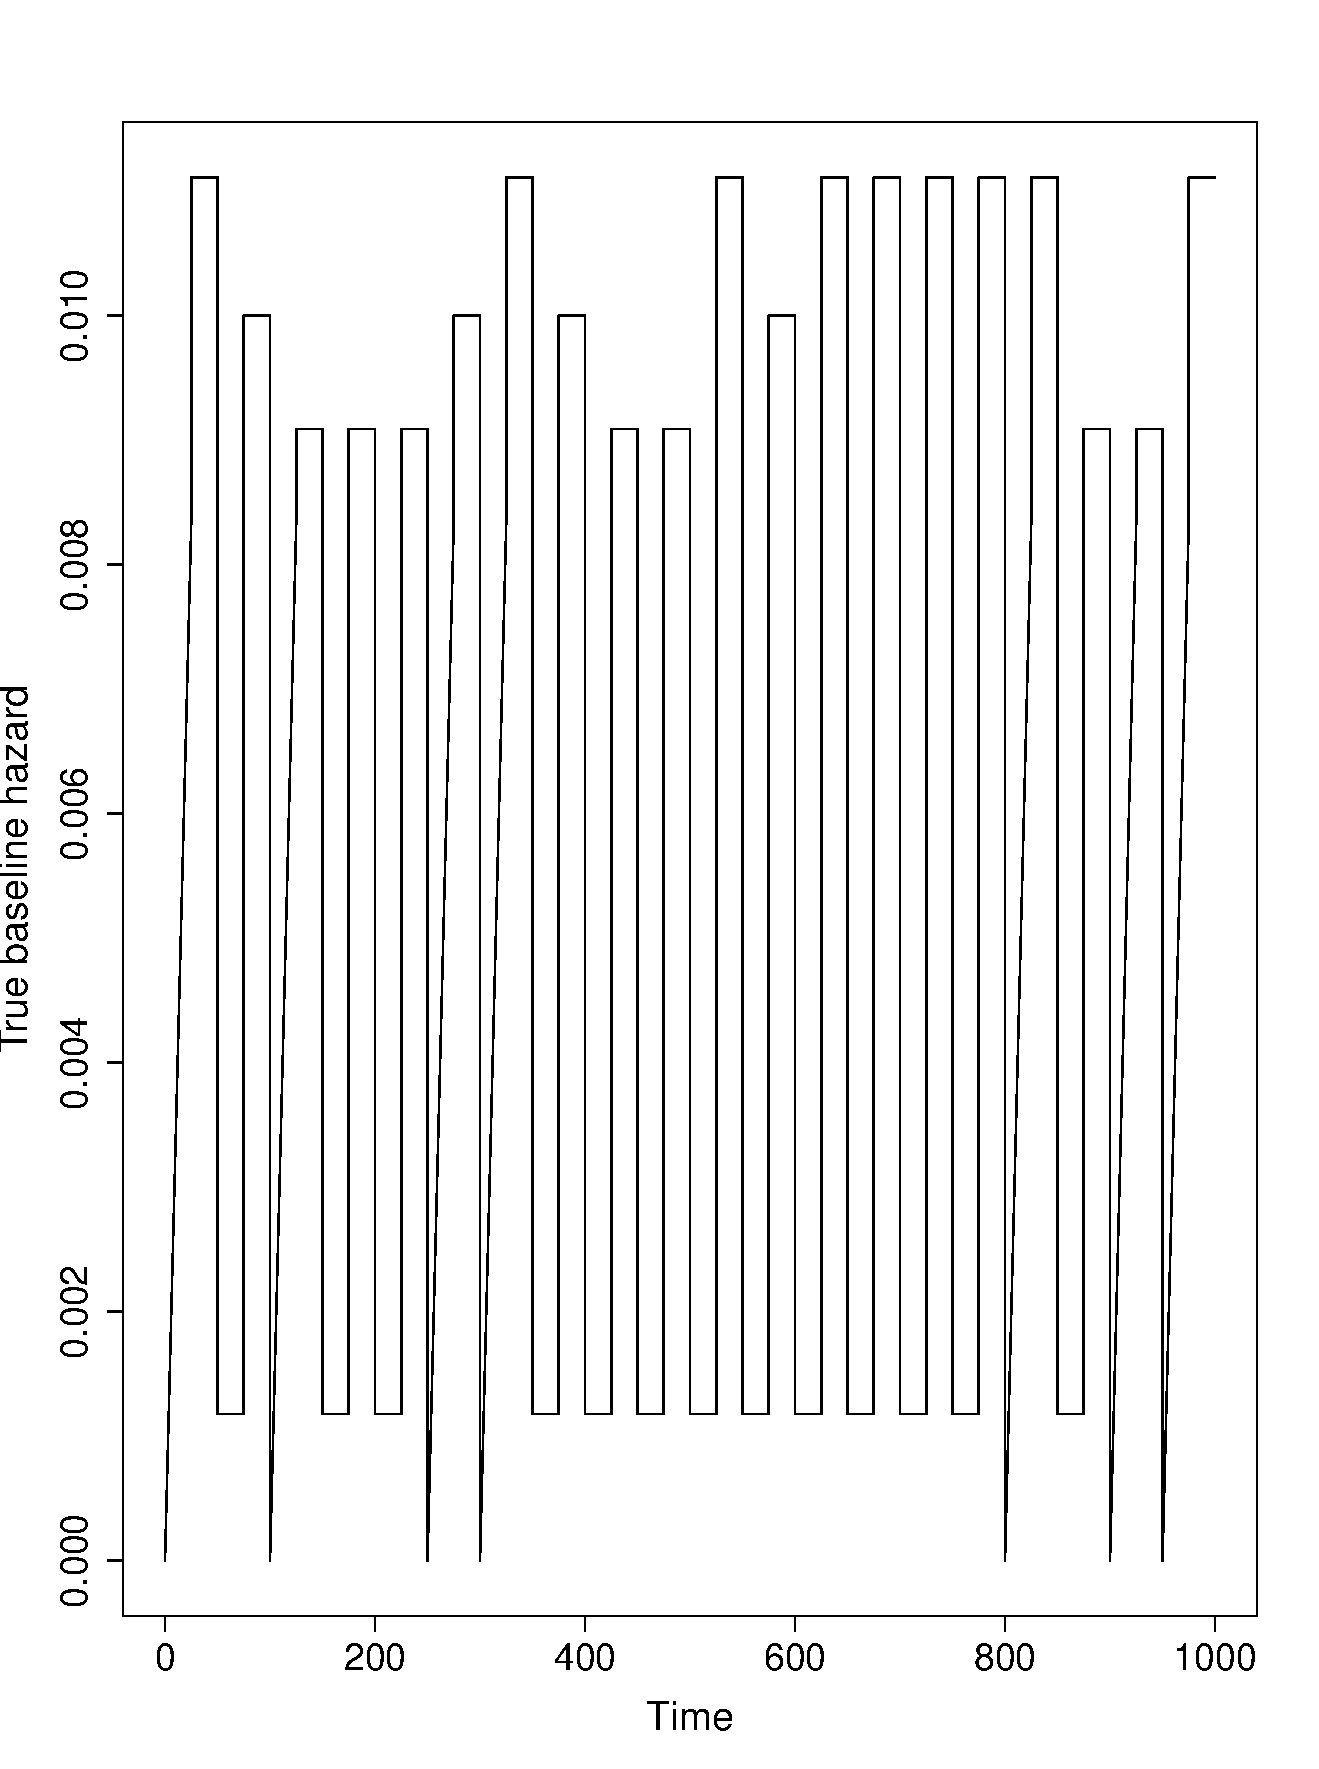
\includegraphics[width=0.45\textwidth,height=3.5in]{sim_base}
}
\subcaptionbox{Posterior for variance parameter $\sigma$}{
	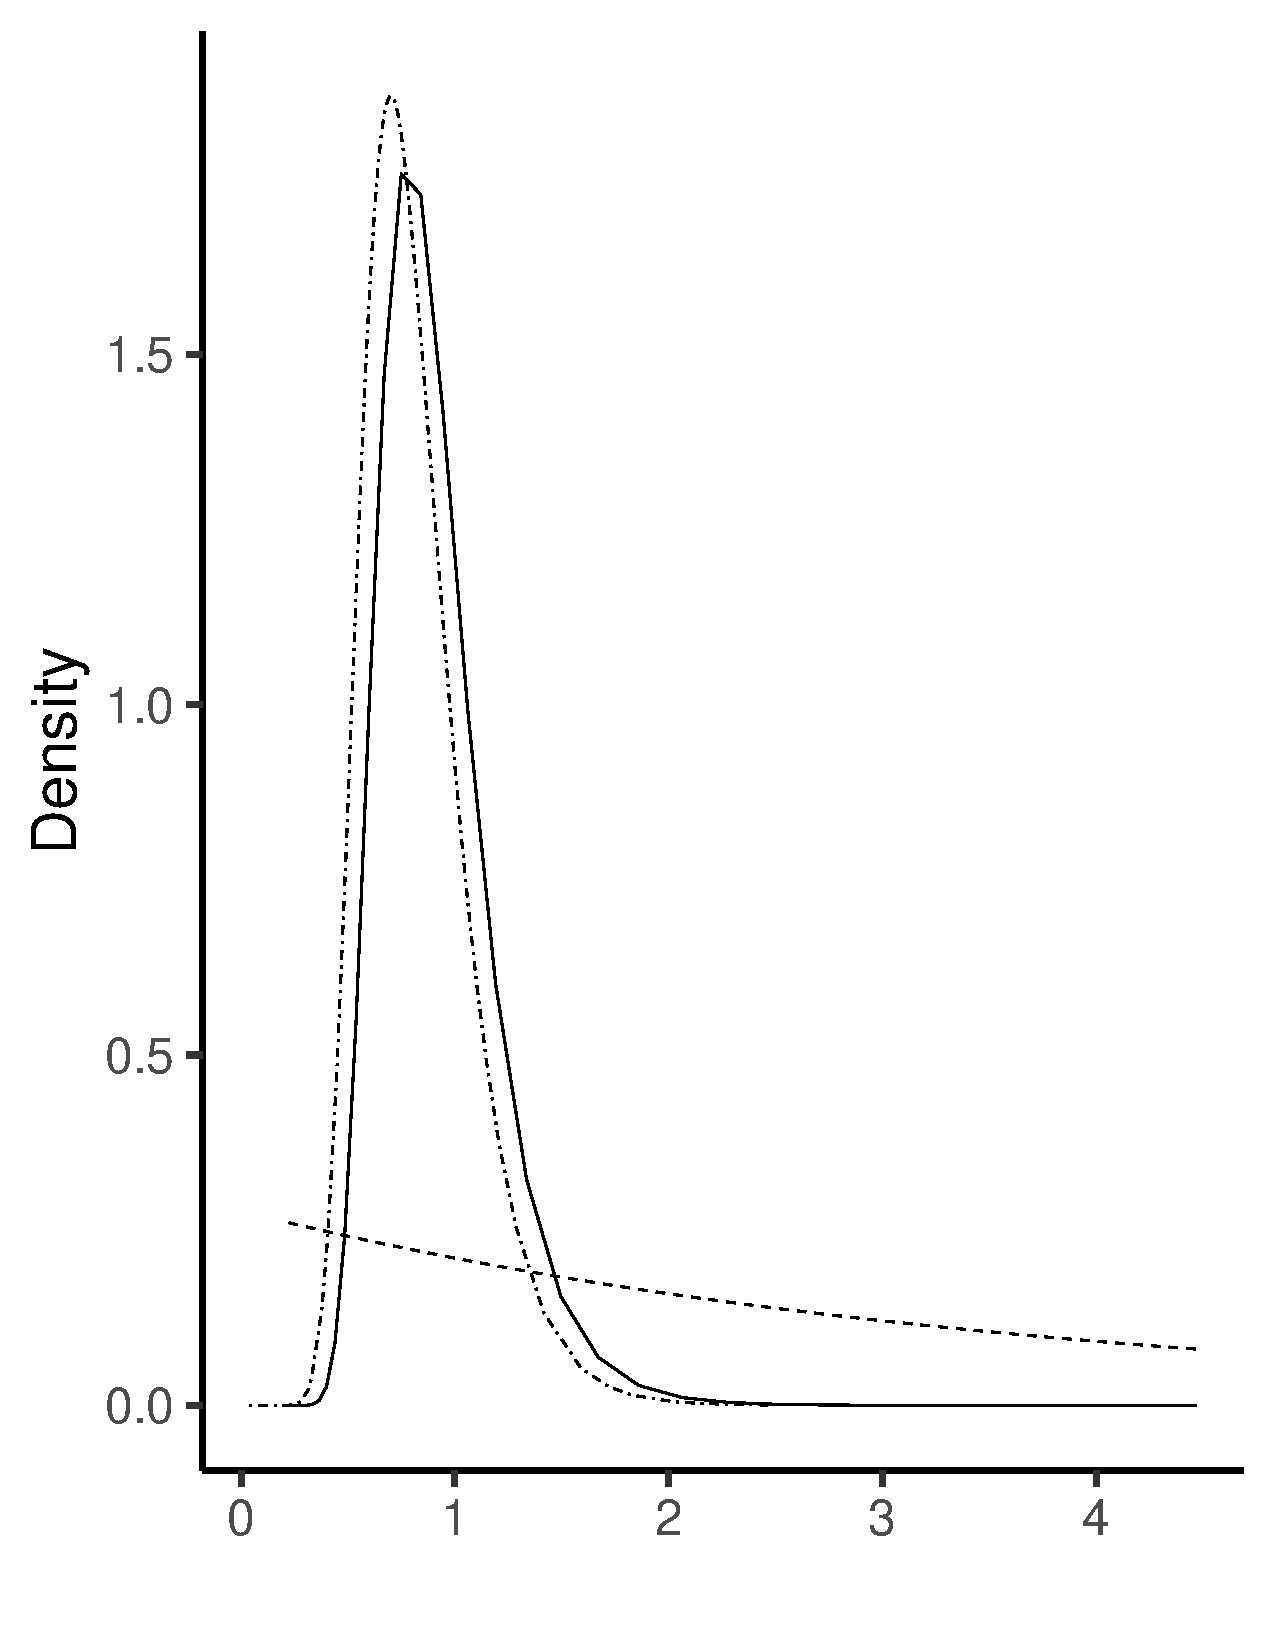
\includegraphics[width=0.45\textwidth,height=3.5in]{SmoothingSim_PosterSigma}
}
\subcaptionbox{Smoothing result}{
	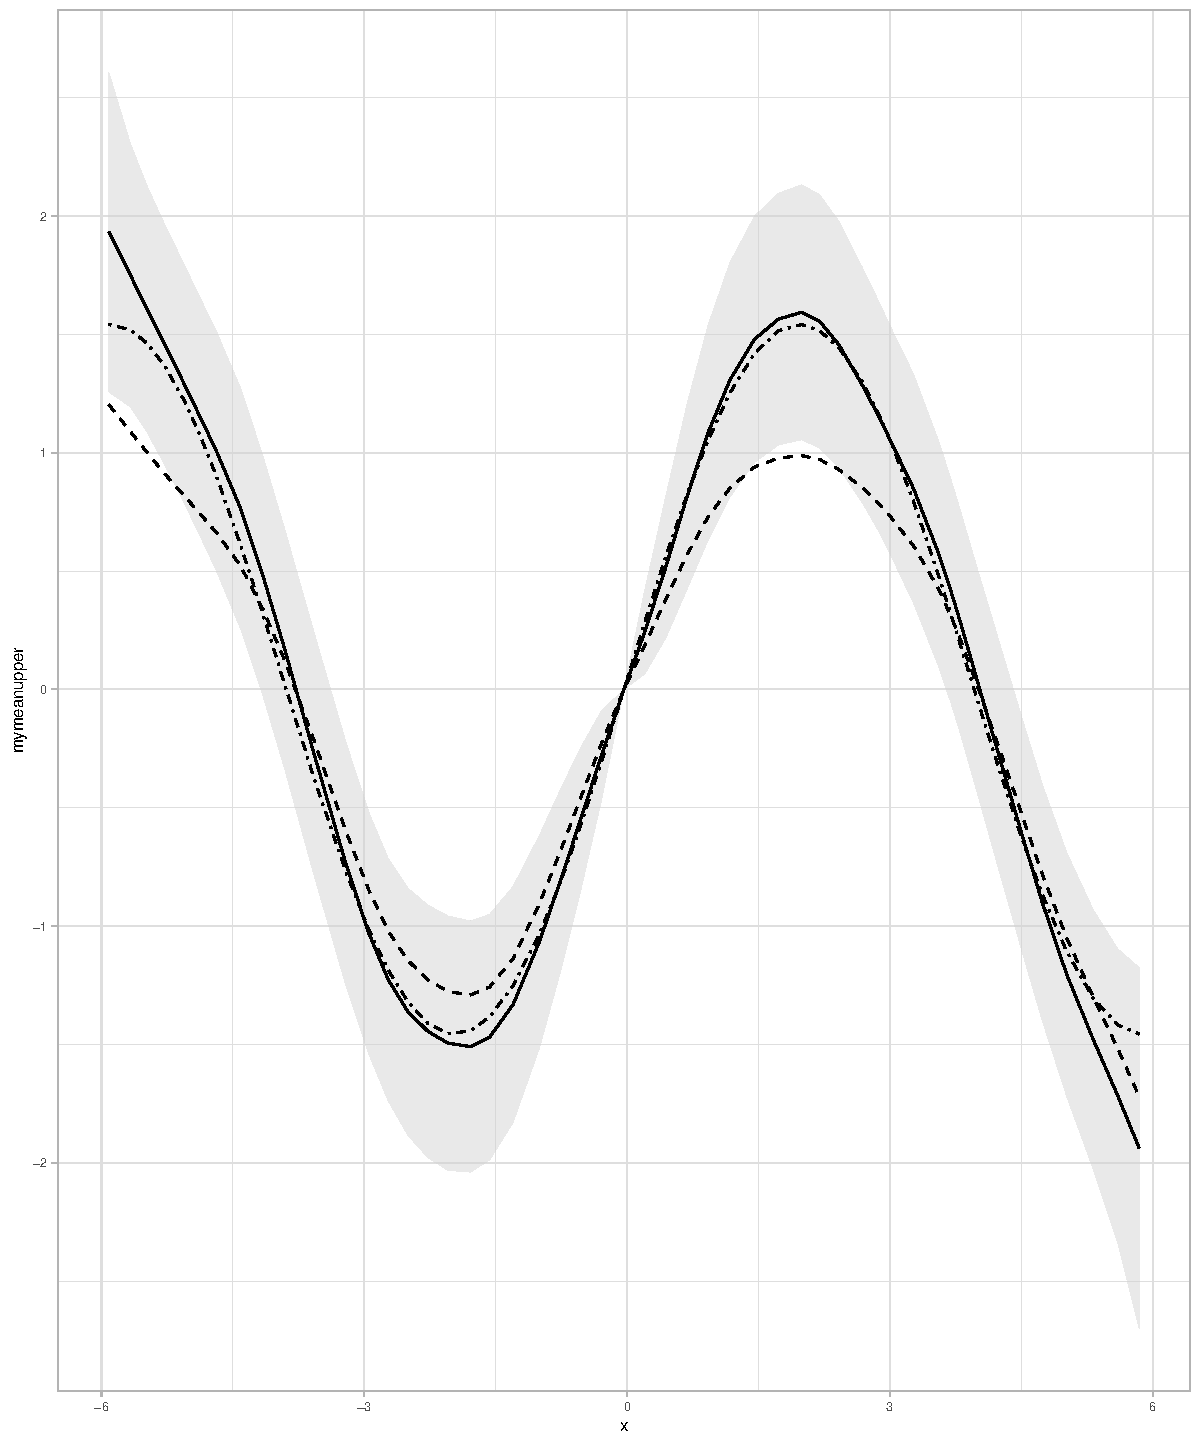
\includegraphics[width=0.45\textwidth,height=3.5in]{SmoothingSim_FinalPlot}
}

\caption{Baseline hazard function in this simulation (top left panel) Posterior Estimation for variance parameter (---) and its prior (- - -)  (top right panels). Bottom panel shows the true risk function (- $\cdot$ -), posterior mean (---) and $95\%$ credible interval using proposed method, posterior mean using INLA (- - -).}
\label{fig:simulation}
\end{figure}

Figure \ref{fig:simulation} demonstrates the superior accuracy of our method over INLA when $h_{0}(t)$ is not smooth. The oscillating baseline hazard could represent a scenario where mortality or morbidity risk varies from day to night, or across days of the week. \alex{can you add the following: 1. INLA's posterior for $\sigma$, on the same plot as ours; 2. INLA's estimated baseline hazard function, on a fourth plot? I need these to be able to further comment on the differences between INLA and us.}

\subsection{Leukaemia Data}

\alex{I think you should take a stab at writing the two data examples sort of like I wrote the above simulation one, and given our discussion where we changed the abstract and clarified the purpose of these two examples. Also, the changes to the plots for the simulation should be reflected in the Leukemia example (basically add their $\sigma$ posterior, on the same graph as ours. For the Kidney example, you should create the tables in Latex using "tabular" and "table" (there is lots of documentation on this). And what's going on with the $\sigma$ posterior in that example? The approximation is convex so the left tail shouldn't inflect like that. Also, INLA's posterior should be shown here too.}

In this example, we will use our proposed methodology to analyse the Leukaemia data set \citet{inlacoxph} did using INLA, and compare these results with the frequentist method GAM. The data set contains 1043 of adult leukaemia patients' information with around 16 percent of them being right-censored. 

For our implementation, we are interested in quantifying the relationship between survival rate of leukaemia patients with the age of the patient ($\text{age}$), the count of white blood cells at diagnosis ($\text{wbc}$), the Townsend deprivation index ($\text{tpi}$) and patient's sex ($\text{sex}$). The effects of $\text{sex}$, $\text{age}$ and $\text{wbc}$ were modelled linearly, and the $\text{tpi}$ was modelled as a semi-parametric smoothing effect. The smoothing variable $\text{tpi}$ was discretized into 50 equally spaced bins. Our methodology does not require the smoothness assumption on the baseline hazard function nor a specification of it.

We set the prior distributions for all the linear effects $\beta$ as $\beta \stackrel{iid}{\sim} \text{N}(0, 0.05^{-1})$, and for the second order random walk of $\Gamma_1 = \{\Gamma_{1,1}, ..., \Gamma_{1,50}\}$ as $\Gamma \sim \text{RW}_2(\sigma^2)$ where a PC prior is put on $\sigma$ such that $\text{P}(\sigma > 3) = 0.5$ \citep{pcprior}. Therefore, the final dimension of W in this example will be 1094. We fit this model using both INLA and our proposed methodology, and then their smoothing results are compared with the result of GAM. For INLA's implementation, it has to assume the smoothness of the baseline hazard and then model it semi-parametrically using random walk model. 

\begin{figure}[ht]
\centering
\subcaptionbox{Posterior for variance parameter $\sigma$}{
	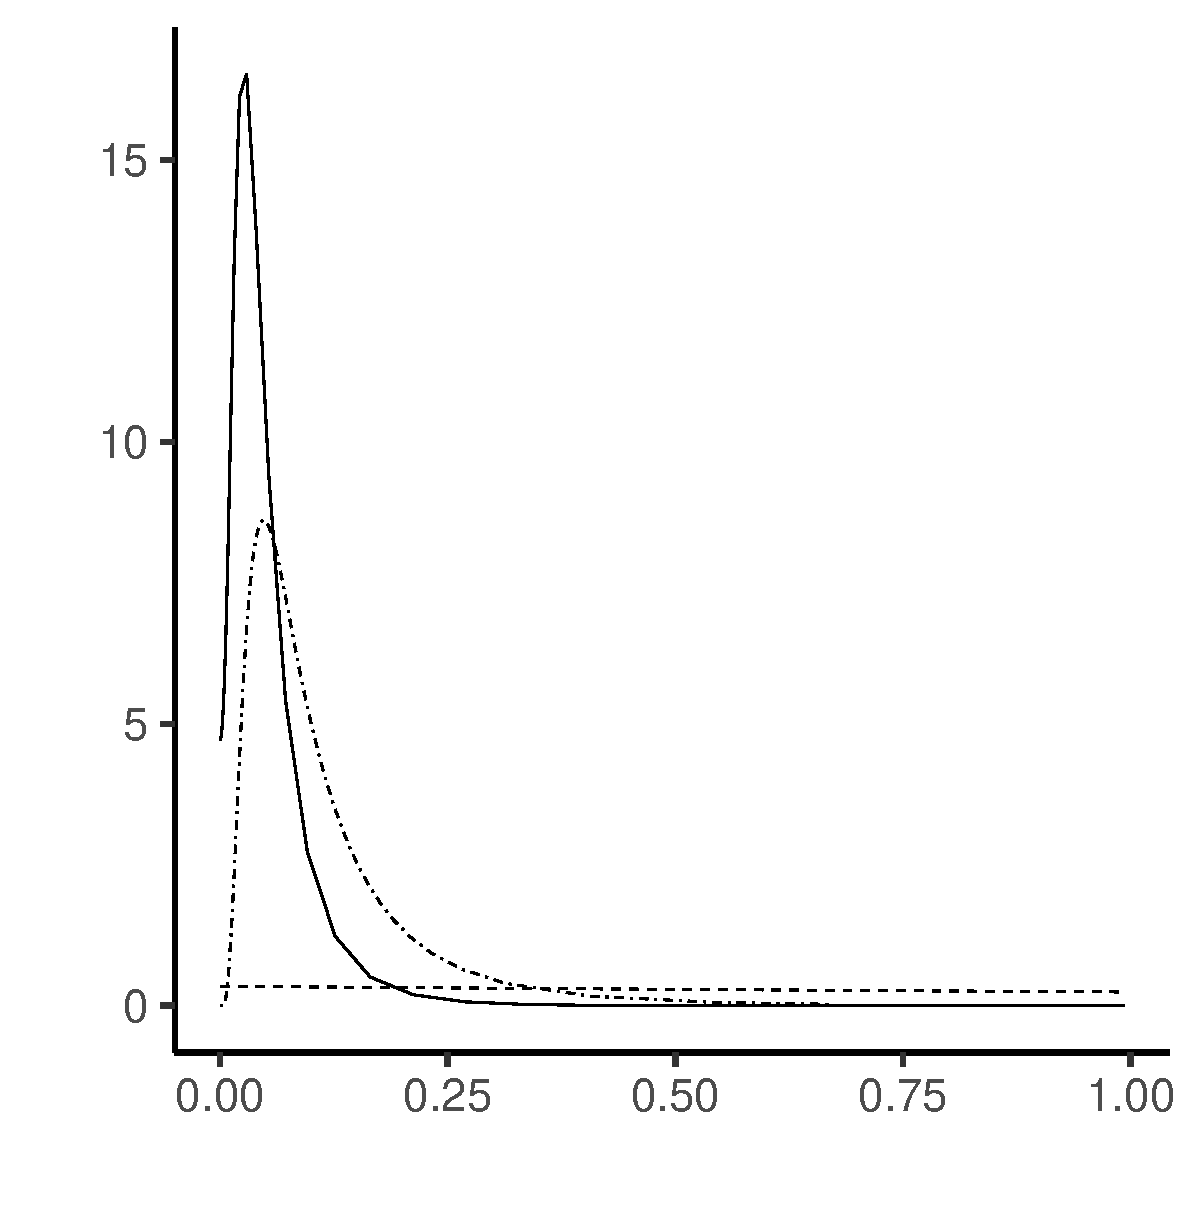
\includegraphics[width=0.45\textwidth,height=3.5in]{Leuk_PosterSigma}
}
\subcaptionbox{Smoothing result}{
	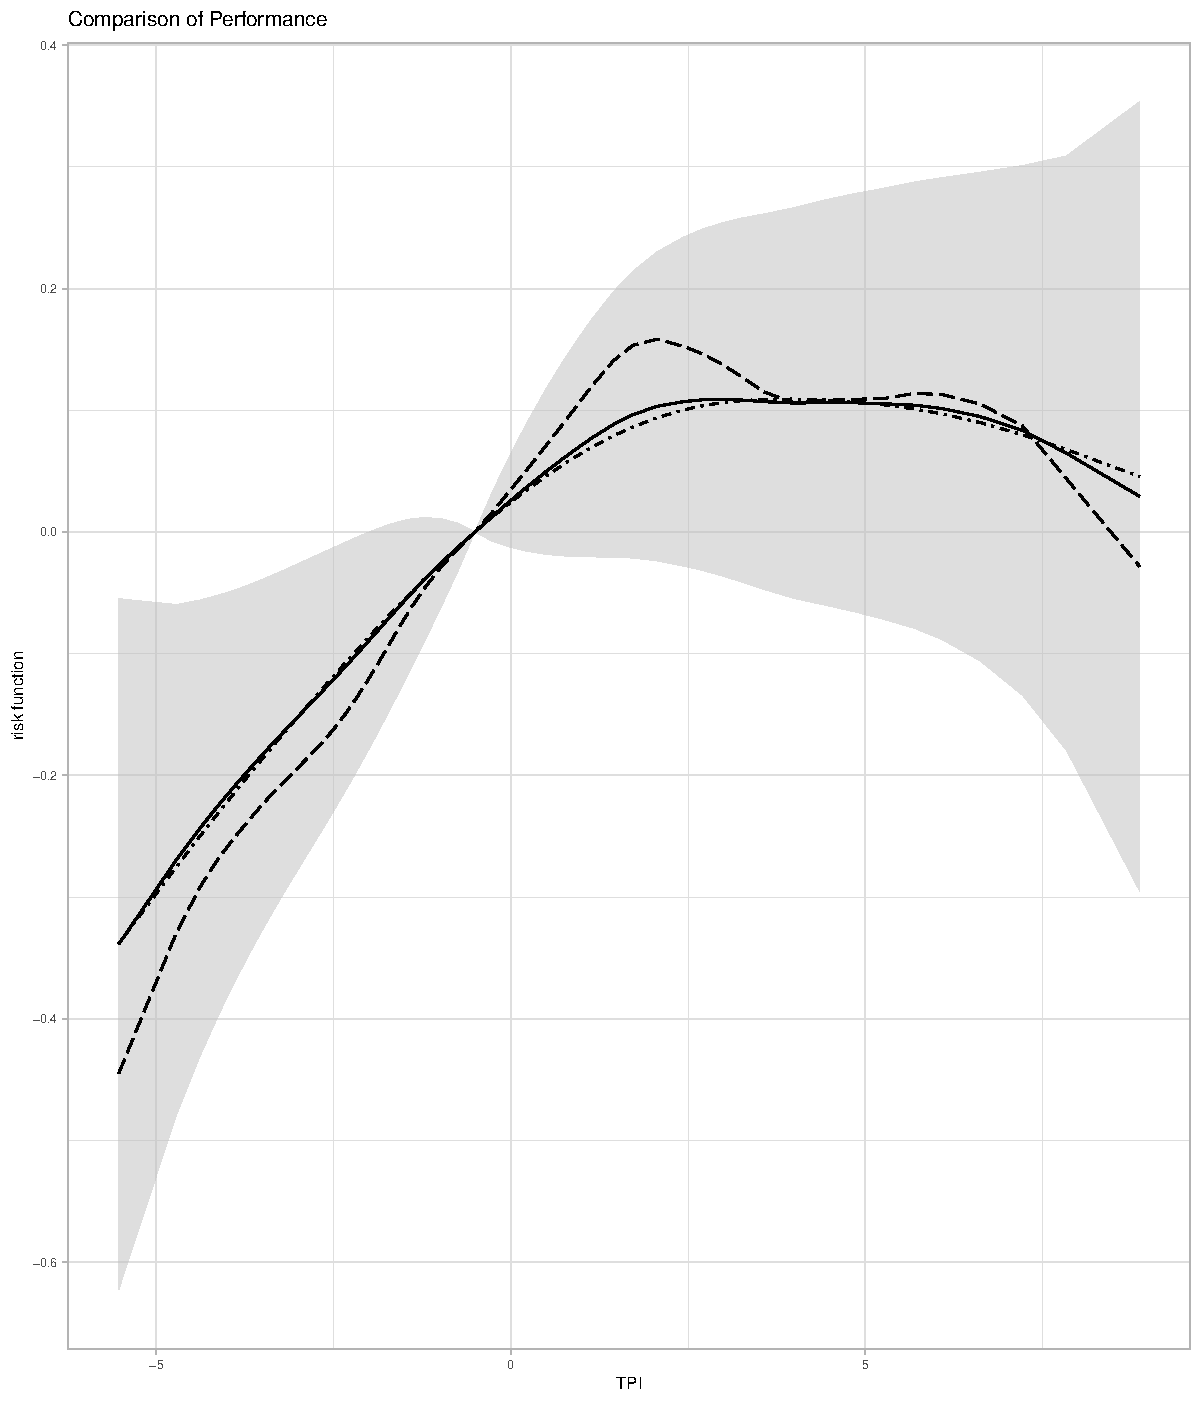
\includegraphics[width=0.45\textwidth,height=3.5in]{leuk_FinalPlot}
}

\caption{Posterior Estimation for variance parameter (---) and its prior (- - -)  (left panel). Right panel shows the posterior mean (---) and $95\%$ credible interval using proposed method, posterior mean using INLA (- - -) and the smoothing result of GAM (- $\cdot$ -).}
\label{fig:leuk}
\end{figure}


Figure \ref{fig:leuk} shows the comparison result of these three methods. It can be seen that the smoothing result given by our method is very similar to the one given by GAM, while the result given by INLA seems comparatively more wiggly. This lack of smoothness may be caused by the inappropriate assumption that INLA put on the form of this baseline hazard function, and in this case it becomes a reason to choose our method or GAM which use the partial likelihood function and hence do not require the specification of the baseline hazard function.

Figure \ref{fig:leuk} shows the posterior distribution of variance parameter given by our algorithm. Based on this plot, it seems like $\sigma$'s value is likely to be very close to zero, which indicates high smoothness on the smoothing function $\Gamma$. This type of model-based quantification of smoothness is a reason to choose Bayesian method over frequentist method such as GAM.


\subsection{Kidney Catheter Data}

In this example, we implement our proposed methodology to analyse the kidney catheter data set that \citet{kidney} analysed using Cox proportional hazard model. This data set contains 76 recurrence times to infection, at the point of insertion of the catheter, for 38 kidney patients. In this data set, each kidney patient has exactly two observations, each observation from one kidney. When the catheter is removed for other reason than infections, the observation is right censored.

In our analysis, we mostly followed the procedures \citet{kidney} did in their work, and aimed to quantify the relationship between recurrence time of bladder infection with patient's age, sex and  disease types. The variable sex is coded as 1 for male and 2 for female. The four diseases types are represented by three dummy variables $\text{GN}$, $\text{AN}$ and $\text{PKD}$, with the reference group being $Other$. A patient level frailty is also added to the model, such that observations within the same patient are correlated. 

We specified the prior distributions for all the linear effect $\beta$ as $\beta \stackrel{iid}{\sim} \text{N}(0, 0.05^{-1})$ , and the prior distribution for the standard deviation of the between-subjects frailty as a PC prior such that $\text{P}(\sigma > 2) = 0.5$. As a comparison, we also implemented INLA and frequentist maximum partial likelihood method for this model. The result is summarized at the figures below.

\begin{figure}[ht]
\centering
\subcaptionbox{Estimated means of linear effects}{
	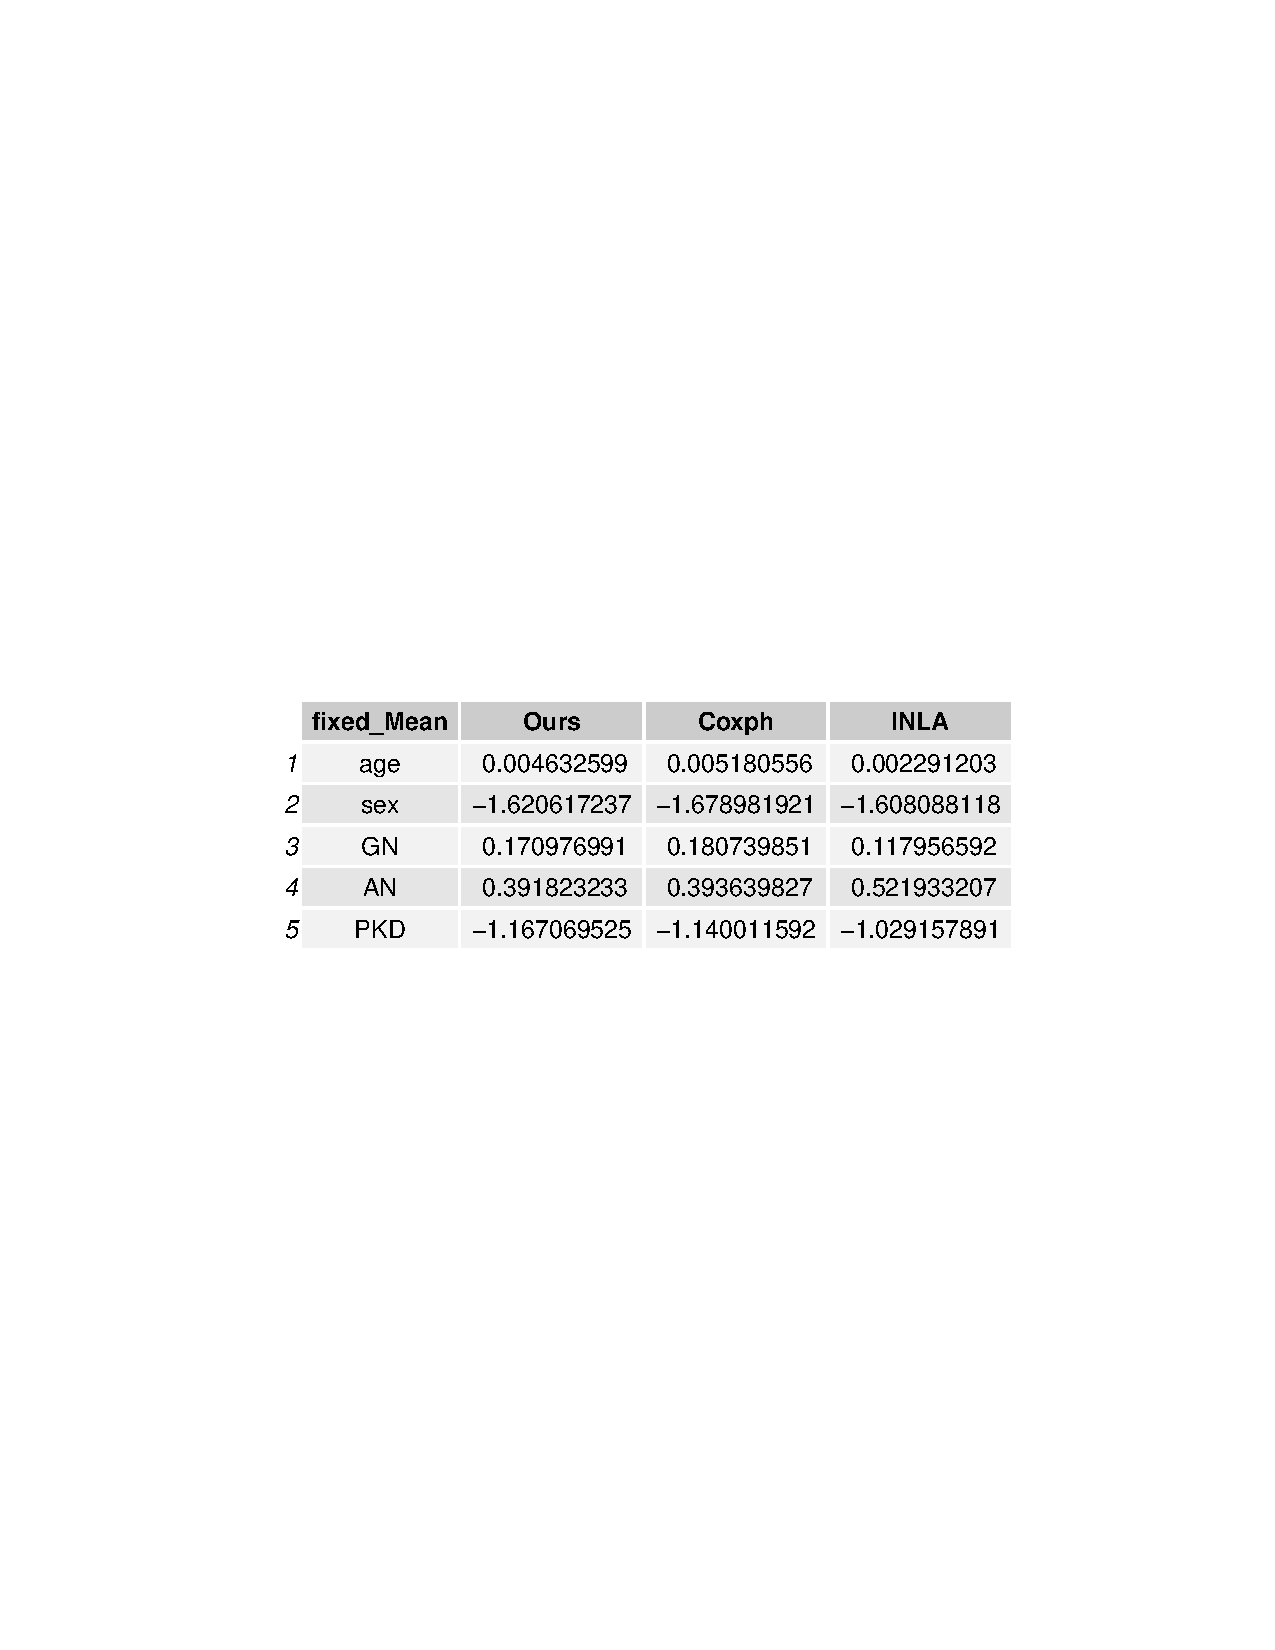
\includegraphics[width=0.75\textwidth,height=3.5in]{FixedEffectsMean}
}
\subcaptionbox{Posterior standard deviations of linear effects }{
	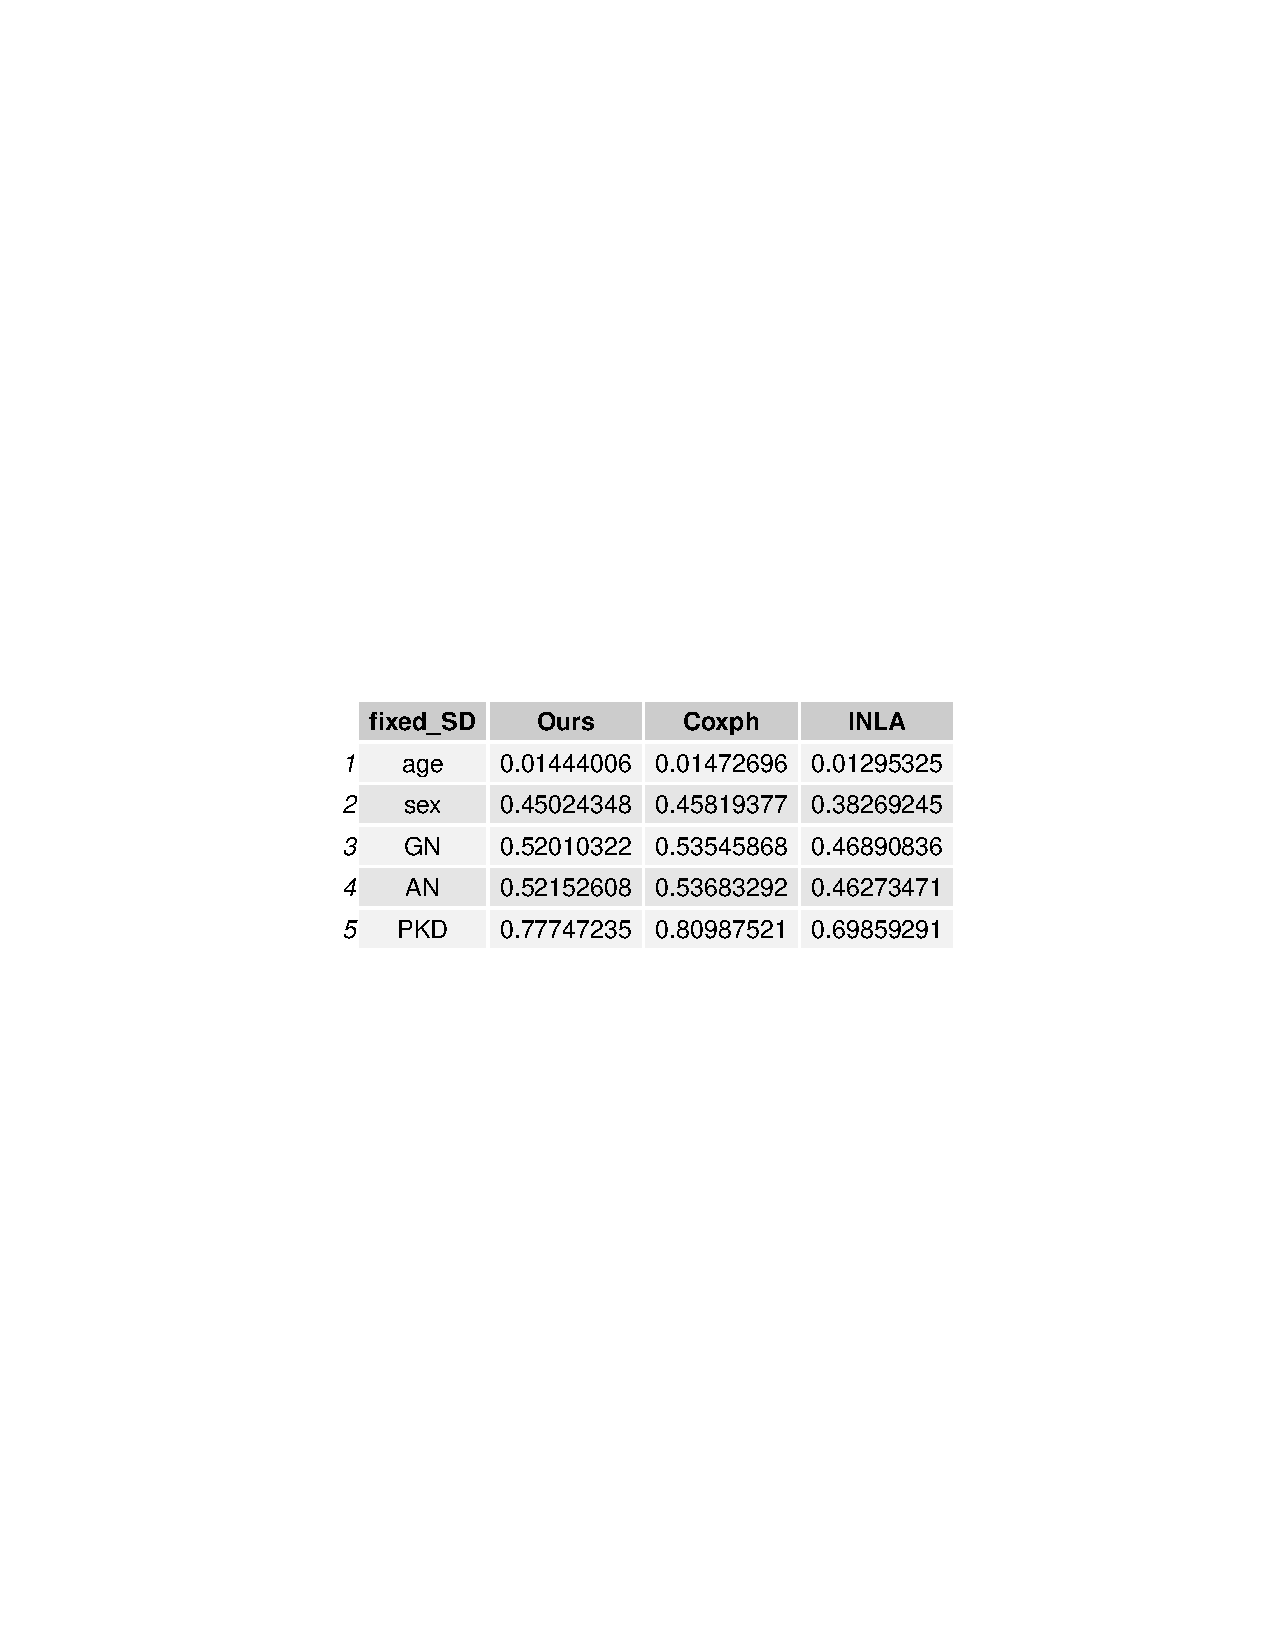
\includegraphics[width=0.75\textwidth,height=3.5in]{FixedEffectsSD}
}
\caption{Posterior Estimation and Maximum Partial likelihood Estimation for linear effects}
\label{fig:BladderLinearEff}
\end{figure}

From figure \ref{fig:BladderLinearEff}, it can be seen that for the inference of linear effects, the posterior means given by our proposed method are very similar to the frequentist's maximum partial likelihood estimates. While the posterior means given by INLA tends to be less similar to the results of the above two methods. Besides that, the posterior standard deviations of these linear effects given by our proposed methods are similar to the estimated standard errors given by maximum partial likelihood methods, but the posterior deviations given by INLA tend to be smaller.

\begin{figure}[ht]
\centering
\subcaptionbox{Posterior for the between-subject standard deviation $\sigma$}{
	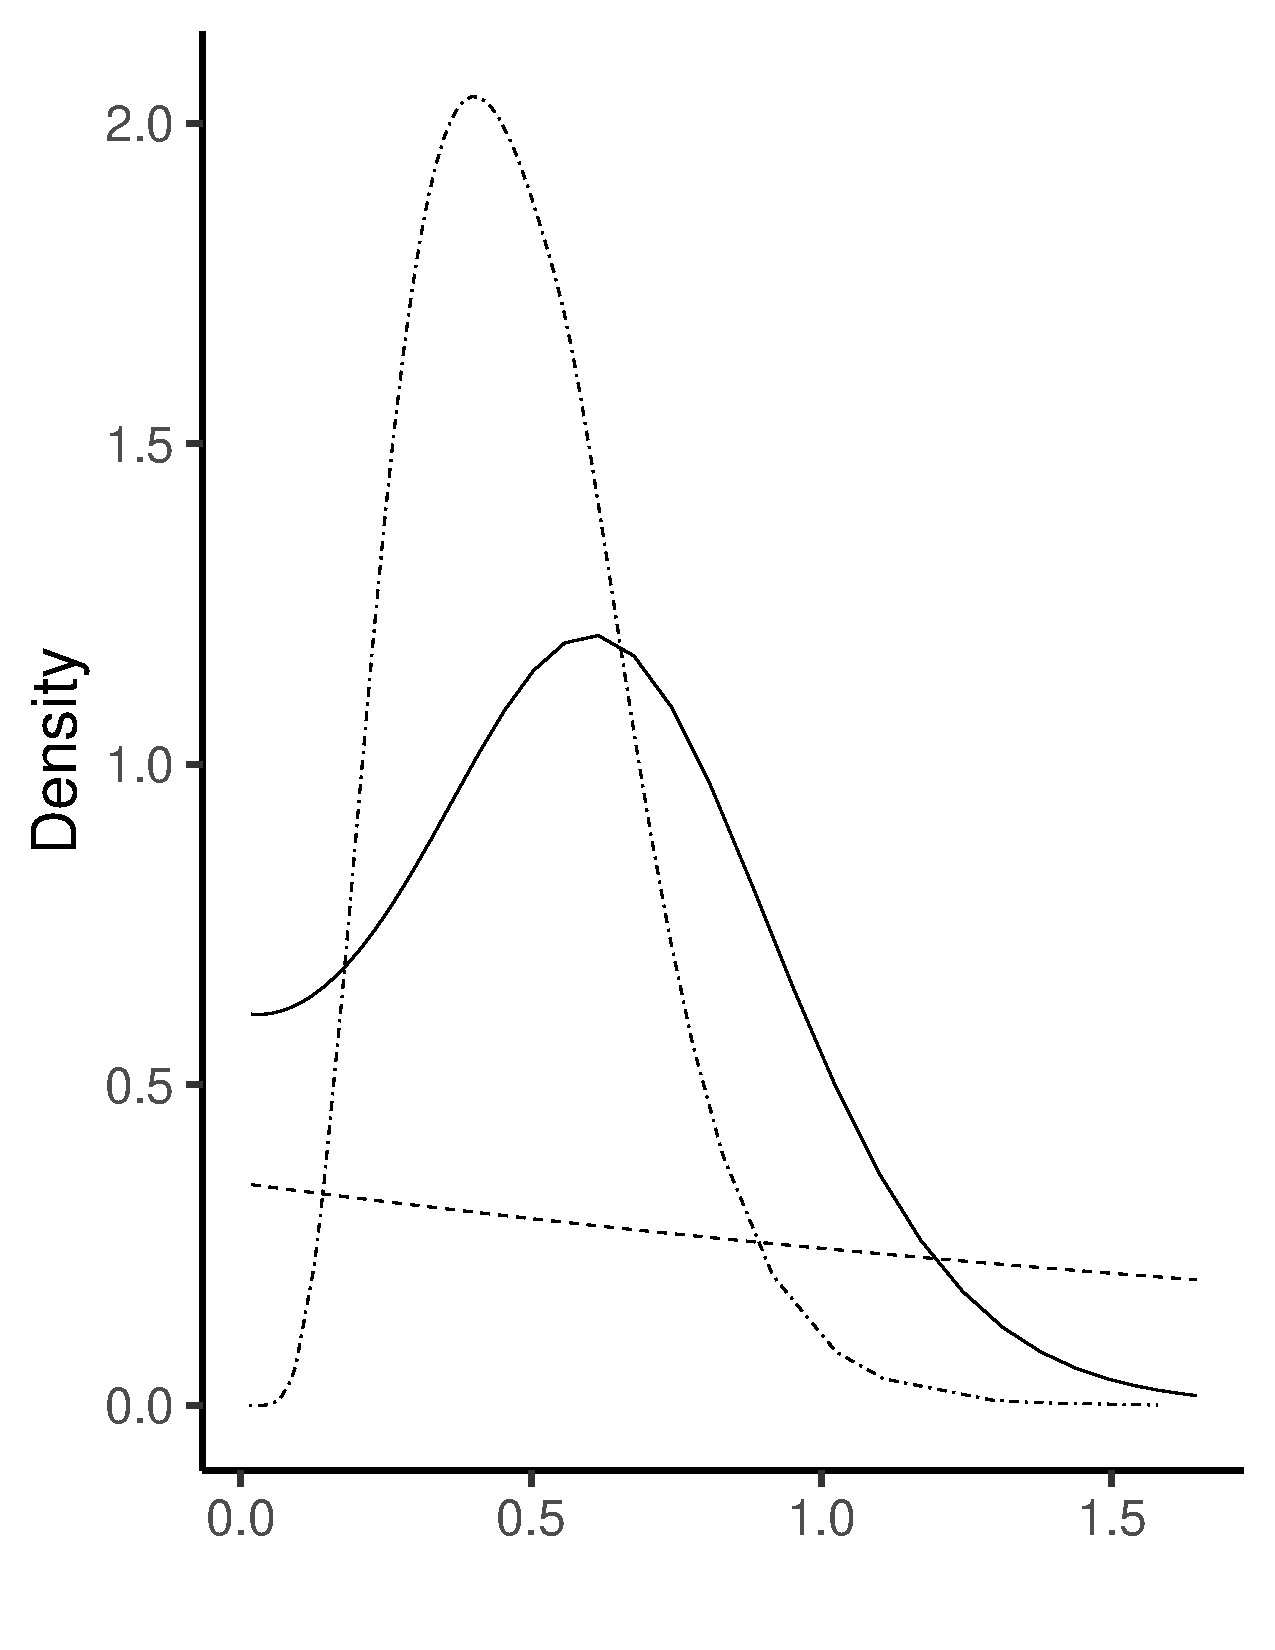
\includegraphics[width=0.45\textwidth,height=3.5in]{Kidney_PosterSigma}
}
\caption{Posterior Estimation for the between-subject standard deviation (---) and its prior (- - -)  (left panel)}
\label{fig:BetweenSubjectSD}
\end{figure}

As contrast to maximum partial likelihood method, our proposed method is able to give a model-based quantification of the between-subject standard deviation $\sigma$. The figure \ref{fig:BetweenSubjectSD} above shows the posterior distribution for the between-subject standard deviation. 



\section{Discussion}\label{sec:discussion}

The novel methodology we proposed in this paper provides a flexible way to do approximate Bayesian inference on Cox proportional hazard model with linear effects, semi-parametric smoothing effects and between-groups frailty. This methodology uses partial likelihood hence does not require the smoothness assumption on the baseline hazard function, which is assumed by INLA as it uses the full likelihood instead. It provides model-based uncertainty quantification of the smoothness parameter and between-groups standard deviation as compared to the bootstrapping method used by frequentist method such as GAM. We have demonstrated its accuracy over alternative approaches through the simulation study, and illustrated its model-based uncertainty quantification through the simulation study and the two real data analysis. As long as the inference on baseline hazard function is of secondary interest, our proposed method will be an appealing option to adopt for the analysis of small to median-size data set.

One limitation of our proposed methodology would be its unscalability to data set with massive size. Since the Hessian matrix in our methodology is fully dense and its number of entries increases quadratically with the sample size, the memory cost will become too heavy for our proposed method to be feasible if the sample size is very large. We avoid the computation of this Hessian matrix during the optimization step by implementing a quasi-Newton method that approximates the true Hessian matrix using update of rank 1, but the true Hessian matrix is still required to be evaluated at the maximum to obtain the posterior inferential result. 

The framework of this proposed methodology can be easily extended to fit more complex model, by modifying the covariance structure of the covariate with semi-parametric effect. For example, adding a covariate with spatially correlated covariance structure such as simultaneously autoregressive model (SAR) can allow the inclusion of spatial effect into the Cox PH model \citep{Spatial}. We will leave these possible extensions to future works.

\newpage

\bibliographystyle{biom}
\bibliography{myrefs}

\appendix

\section{Derivation of Precision Matrix}

In this seciton we give a brief derivation of the precision matrix $Q_{\theta}$ from Equation ... The derivation is identical to that of \citet{casecross} (Web Appendix C), with a different differencing matrix. The differencing matrix $D$ is:
\begin{equation}\begin{aligned}\label{eqn:D2}
D &= \begin{pmatrix}
1 & -1 & 0 & \cdots & 0 \\
1 & 0 & -1 & \cdots & 0 \\
  &    & \ddots &   &   \\
1 &    &       & 0 & -1 \\
\end{pmatrix}
\end{aligned}\end{equation}
Our model specifies:
\begin{equation*}
\Gamma|\theta \sim \text{Normal}\left( 0,\Sigma_{\Gamma}\right); \ \beta \sim \text{Normal}\left( 0,\Sigma_{\beta}\right); \ \epsilon \sim \text{Normal}\left( 0,\tau^{-1}I\right)
\end{equation*}
all independent of each other, and of $\theta$ unless otherwise specified. The additive predictor is $\eta = A\Gamma + X\beta + \epsilon$ and $\Delta = D\eta$ where $D$ is defined through Equation .... This gives a joint distribution for $W|\theta$:
\begin{equation*}
W|\theta = \begin{pmatrix} \Delta \\ \Gamma \\\beta \end{pmatrix} = \begin{pmatrix} DA & DX & D \\ I & 0 & 0 \\ 0 & I & 0 \\ \end{pmatrix}\begin{pmatrix}\Gamma \\ \beta \\ \epsilon \end{pmatrix} 
\sim \text{Normal}\left( 0,\Sigma\right)
\end{equation*}
where
\begin{equation*}
\Sigma = \begin{pmatrix}
DA\Sigma_{\Gamma}A^{T}D^{T} + DX\Sigma_{\beta}X^{T}D^{T} + \tau^{-1}DD^{T} & DA\Sigma_{\Gamma} & DX\Sigma_{\beta} \\
\Sigma_{\Gamma}D^{T}A^{T} & \Sigma_{\Gamma} & 0 \\
\Sigma_{\beta}D^{T}X^{T} & 0 & \Sigma_{\beta} \\
\end{pmatrix}
\end{equation*}
Direct calculation using formuals for block matrix inversion yields $Q(\theta) = \Sigma^{-1}$.



\end{document}